\documentclass[1p]{elsarticle_modified}
%\bibliographystyle{elsarticle-num}

%\usepackage[colorlinks]{hyperref}
%\usepackage{abbrmath_seonhwa} %\Abb, \Ascr, \Acal ,\Abf, \Afrak
\usepackage{amsfonts}
\usepackage{amssymb}
\usepackage{amsmath}
\usepackage{amsthm}
\usepackage{scalefnt}
\usepackage{amsbsy}
\usepackage{kotex}
\usepackage{caption}
\usepackage{subfig}
\usepackage{color}
\usepackage{graphicx}
\usepackage{xcolor} %% white, black, red, green, blue, cyan, magenta, yellow
\usepackage{float}
\usepackage{setspace}
\usepackage{hyperref}

\usepackage{tikz}
\usetikzlibrary{arrows}

\usepackage{multirow}
\usepackage{array} % fixed length table
\usepackage{hhline}

%%%%%%%%%%%%%%%%%%%%%
\makeatletter
\renewcommand*\env@matrix[1][\arraystretch]{%
	\edef\arraystretch{#1}%
	\hskip -\arraycolsep
	\let\@ifnextchar\new@ifnextchar
	\array{*\c@MaxMatrixCols c}}
\makeatother %https://tex.stackexchange.com/questions/14071/how-can-i-increase-the-line-spacing-in-a-matrix
%%%%%%%%%%%%%%%

\usepackage[normalem]{ulem}

\newcommand{\msout}[1]{\ifmmode\text{\sout{\ensuremath{#1}}}\else\sout{#1}\fi}
%SOURCE: \msout is \stkout macro in https://tex.stackexchange.com/questions/20609/strikeout-in-math-mode

\newcommand{\cancel}[1]{
	\ifmmode
	{\color{red}\msout{#1}}
	\else
	{\color{red}\sout{#1}}
	\fi
}

\newcommand{\add}[1]{
	{\color{blue}\uwave{#1}}
}

\newcommand{\replace}[2]{
	\ifmmode
	{\color{red}\msout{#1}}{\color{blue}\uwave{#2}}
	\else
	{\color{red}\sout{#1}}{\color{blue}\uwave{#2}}
	\fi
}

\newcommand{\Sol}{\mathcal{S}} %segment
\newcommand{\D}{D} %diagram
\newcommand{\A}{\mathcal{A}} %arc


%%%%%%%%%%%%%%%%%%%%%%%%%%%%%5 test

\def\sl{\operatorname{\textup{SL}}(2,\Cbb)}
\def\psl{\operatorname{\textup{PSL}}(2,\Cbb)}
\def\quan{\mkern 1mu \triangleright \mkern 1mu}

\theoremstyle{definition}
\newtheorem{thm}{Theorem}[section]
\newtheorem{prop}[thm]{Proposition}
\newtheorem{lem}[thm]{Lemma}
\newtheorem{ques}[thm]{Question}
\newtheorem{cor}[thm]{Corollary}
\newtheorem{defn}[thm]{Definition}
\newtheorem{exam}[thm]{Example}
\newtheorem{rmk}[thm]{Remark}
\newtheorem{alg}[thm]{Algorithm}

\newcommand{\I}{\sqrt{-1}}
\begin{document}

%\begin{frontmatter}
%
%\title{Boundary parabolic representations of knots up to 8 crossings}
%
%%% Group authors per affiliation:
%\author{Yunhi Cho} 
%\address{Department of Mathematics, University of Seoul, Seoul, Korea}
%\ead{yhcho@uos.ac.kr}
%
%
%\author{Seonhwa Kim} %\fnref{s_kim}}
%\address{Center for Geometry and Physics, Institute for Basic Science, Pohang, 37673, Korea}
%\ead{ryeona17@ibs.re.kr}
%
%\author{Hyuk Kim}
%\address{Department of Mathematical Sciences, Seoul National University, Seoul 08826, Korea}
%\ead{hyukkim@snu.ac.kr}
%
%\author{Seokbeom Yoon}
%\address{Department of Mathematical Sciences, Seoul National University, Seoul, 08826,  Korea}
%\ead{sbyoon15@snu.ac.kr}
%
%\begin{abstract}
%We find all boundary parabolic representation of knots up to 8 crossings.
%
%\end{abstract}
%\begin{keyword}
%    \MSC[2010] 57M25 
%\end{keyword}
%
%\end{frontmatter}

%\linenumbers
%\tableofcontents
%
\newcommand\colored[1]{\textcolor{white}{\rule[-0.35ex]{0.8em}{1.4ex}}\kern-0.8em\color{red} #1}%
%\newcommand\colored[1]{\textcolor{white}{ #1}\kern-2.17ex	\textcolor{white}{ #1}\kern-1.81ex	\textcolor{white}{ #1}\kern-2.15ex\color{red}#1	}

{\Large $\underline{12n_{0422}~(K12n_{0422})}$}

\setlength{\tabcolsep}{10pt}
\renewcommand{\arraystretch}{1.6}
\vspace{1cm}\begin{tabular}{m{100pt}>{\centering\arraybackslash}m{274pt}}
\multirow{5}{120pt}{
	\centering
	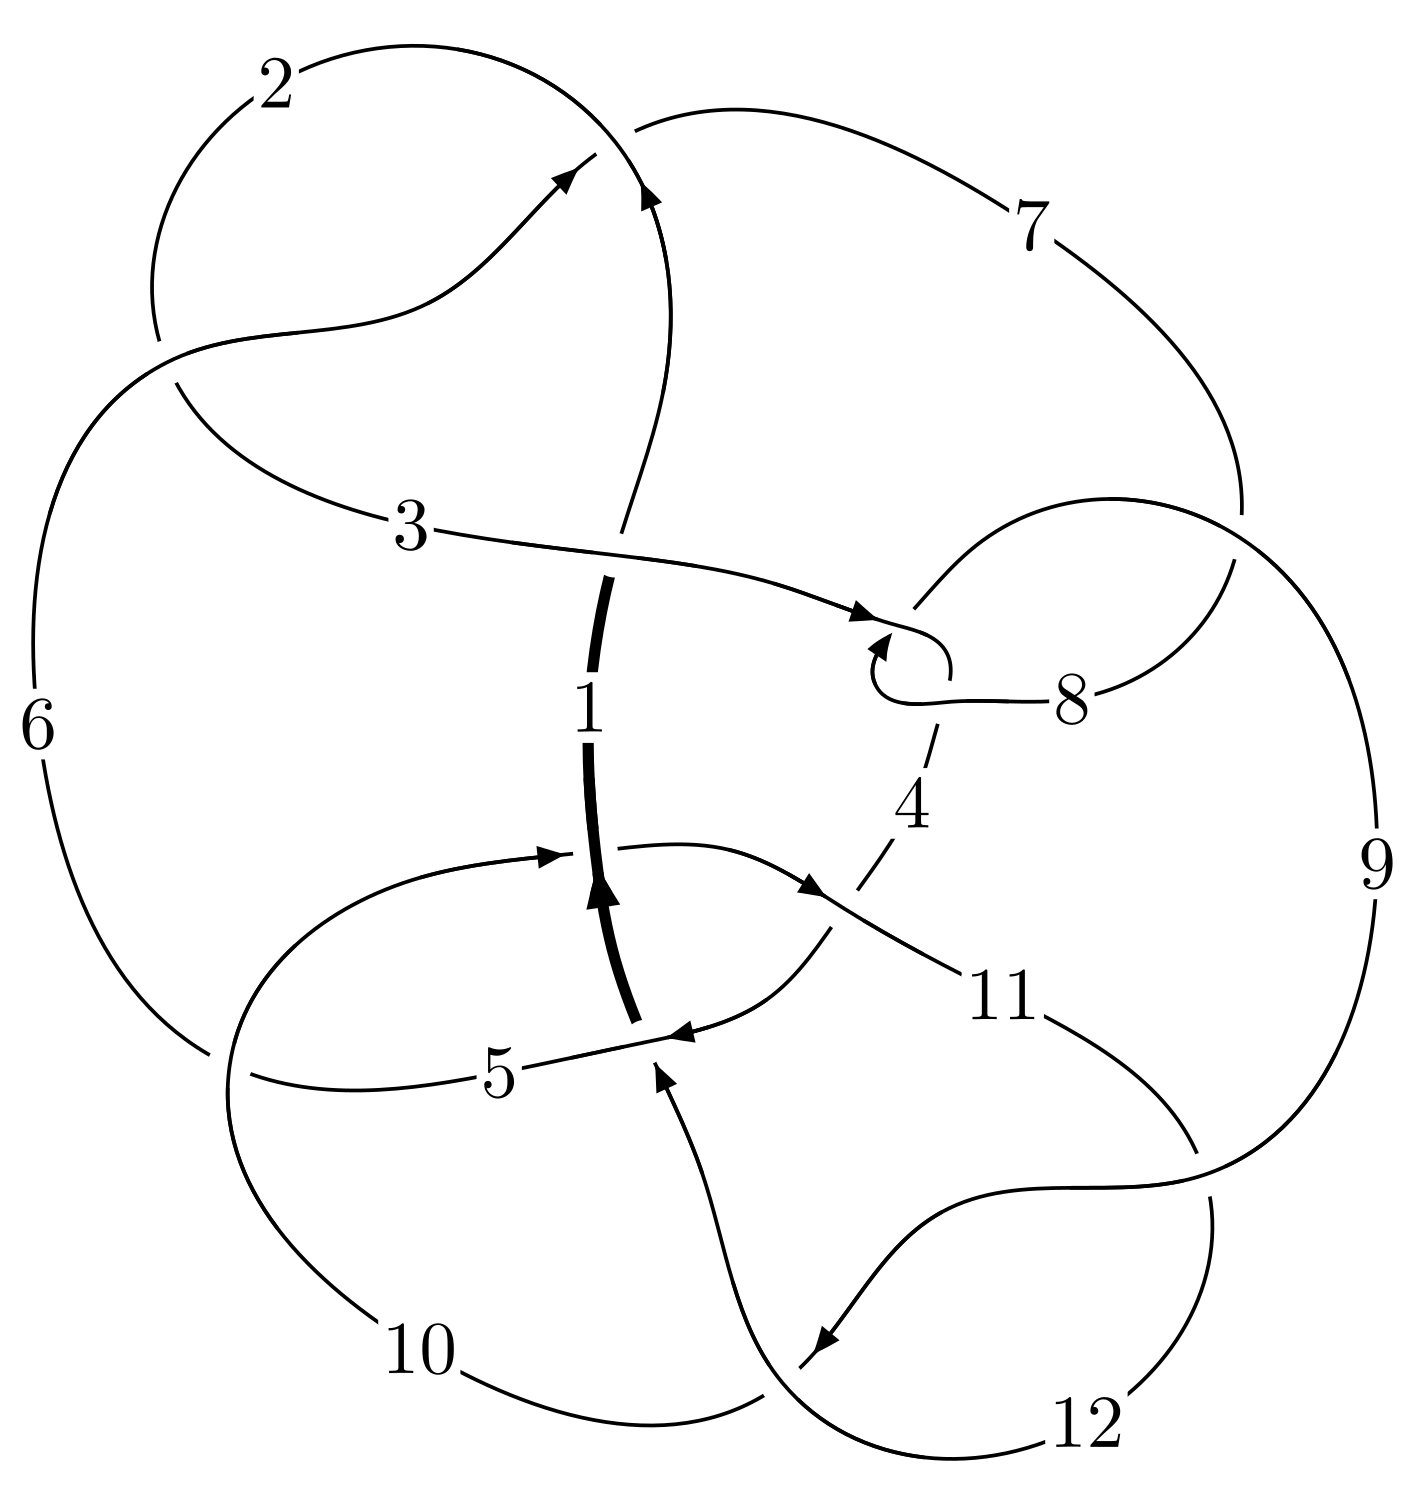
\includegraphics[width=112pt]{../../../GIT/diagram.site/Diagrams/png/2511_12n_0422.png}\\
\ \ \ A knot diagram\footnotemark}&
\allowdisplaybreaks
\textbf{Linearized knot diagam} \\
\cline{2-2}
 &
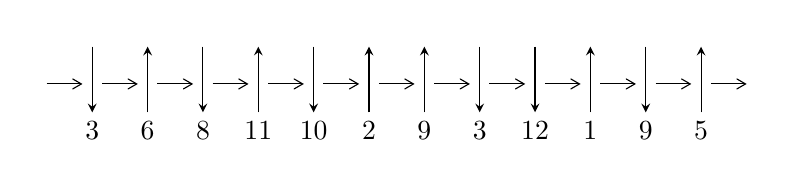
\begin{tikzpicture}[x=20pt, y=17pt]
	% nodes
	\node (C0) at (0, 0) {};
	\node (C1) at (1, 0) {};
	\node (C1U) at (1, +1) {};
	\node (C1D) at (1, -1) {3};

	\node (C2) at (2, 0) {};
	\node (C2U) at (2, +1) {};
	\node (C2D) at (2, -1) {6};

	\node (C3) at (3, 0) {};
	\node (C3U) at (3, +1) {};
	\node (C3D) at (3, -1) {8};

	\node (C4) at (4, 0) {};
	\node (C4U) at (4, +1) {};
	\node (C4D) at (4, -1) {11};

	\node (C5) at (5, 0) {};
	\node (C5U) at (5, +1) {};
	\node (C5D) at (5, -1) {10};

	\node (C6) at (6, 0) {};
	\node (C6U) at (6, +1) {};
	\node (C6D) at (6, -1) {2};

	\node (C7) at (7, 0) {};
	\node (C7U) at (7, +1) {};
	\node (C7D) at (7, -1) {9};

	\node (C8) at (8, 0) {};
	\node (C8U) at (8, +1) {};
	\node (C8D) at (8, -1) {3};

	\node (C9) at (9, 0) {};
	\node (C9U) at (9, +1) {};
	\node (C9D) at (9, -1) {12};

	\node (C10) at (10, 0) {};
	\node (C10U) at (10, +1) {};
	\node (C10D) at (10, -1) {1};

	\node (C11) at (11, 0) {};
	\node (C11U) at (11, +1) {};
	\node (C11D) at (11, -1) {9};

	\node (C12) at (12, 0) {};
	\node (C12U) at (12, +1) {};
	\node (C12D) at (12, -1) {5};
	\node (C13) at (13, 0) {};

	% arrows
	\draw[->,>={angle 60}]
	(C0) edge (C1) (C1) edge (C2) (C2) edge (C3) (C3) edge (C4) (C4) edge (C5) (C5) edge (C6) (C6) edge (C7) (C7) edge (C8) (C8) edge (C9) (C9) edge (C10) (C10) edge (C11) (C11) edge (C12) (C12) edge (C13) ;	\draw[->,>=stealth]
	(C1U) edge (C1D) (C2D) edge (C2U) (C3U) edge (C3D) (C4D) edge (C4U) (C5U) edge (C5D) (C6D) edge (C6U) (C7D) edge (C7U) (C8U) edge (C8D) (C9U) edge (C9D) (C10D) edge (C10U) (C11U) edge (C11D) (C12D) edge (C12U) ;
	\end{tikzpicture} \\
\hhline{~~} \\& 
\textbf{Solving Sequence} \\ \cline{2-2} 
 &
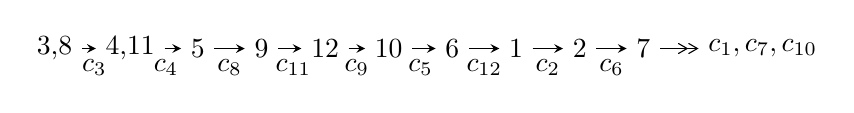
\begin{tikzpicture}[x=23pt, y=7pt]
	% node
	\node (A0) at (-1/8, 0) {3,8};
	\node (A1) at (17/16, 0) {4,11};
	\node (A2) at (17/8, 0) {5};
	\node (A3) at (25/8, 0) {9};
	\node (A4) at (33/8, 0) {12};
	\node (A5) at (41/8, 0) {10};
	\node (A6) at (49/8, 0) {6};
	\node (A7) at (57/8, 0) {1};
	\node (A8) at (65/8, 0) {2};
	\node (A9) at (73/8, 0) {7};
	\node (C1) at (1/2, -1) {$c_{3}$};
	\node (C2) at (13/8, -1) {$c_{4}$};
	\node (C3) at (21/8, -1) {$c_{8}$};
	\node (C4) at (29/8, -1) {$c_{11}$};
	\node (C5) at (37/8, -1) {$c_{9}$};
	\node (C6) at (45/8, -1) {$c_{5}$};
	\node (C7) at (53/8, -1) {$c_{12}$};
	\node (C8) at (61/8, -1) {$c_{2}$};
	\node (C9) at (69/8, -1) {$c_{6}$};
	\node (A10) at (11, 0) {$c_{1},c_{7},c_{10}$};

	% edge
	\draw[->,>=stealth]	
	(A0) edge (A1) (A1) edge (A2) (A2) edge (A3) (A3) edge (A4) (A4) edge (A5) (A5) edge (A6) (A6) edge (A7) (A7) edge (A8) (A8) edge (A9) ;
	\draw[->>,>={angle 60}]	
	(A9) edge (A10);
\end{tikzpicture} \\ 

\end{tabular} \\

\footnotetext{
The image of knot diagram is generated by the software ``\textbf{Draw programme}" developed by Andrew Bartholomew(\url{http://www.layer8.co.uk/maths/draw/index.htm\#Running-draw}), where we modified some parts for our purpose(\url{https://github.com/CATsTAILs/LinksPainter}).
}\phantom \\ \newline 
\centering \textbf{Ideals for irreducible components\footnotemark of $X_{\text{par}}$} 
 
\begin{align*}
I^u_{1}&=\langle 
-8.28749\times10^{71} u^{53}-2.33614\times10^{73} u^{52}+\cdots+3.81141\times10^{75} b+2.99444\times10^{75},\\
\phantom{I^u_{1}}&\phantom{= \langle  }-5.98664\times10^{75} u^{53}+1.19971\times10^{76} u^{52}+\cdots+6.47940\times10^{76} a+3.22020\times10^{76},\\
\phantom{I^u_{1}}&\phantom{= \langle  }u^{54}-2 u^{53}+\cdots-112 u+17\rangle \\
I^u_{2}&=\langle 
-58 u^{17}-4 u^{16}+\cdots+69 b-127 u,\;4 u^{16}-58 u^{15}+\cdots+69 a-220,\;u^{18}+6 u^{16}+\cdots+3 u+1\rangle \\
I^u_{3}&=\langle 
-4 a^4 u+18 a^3 u+16 a^3+9 a^2 u-54 a^2-52 a u+5 b+19 a+13 u+16,\\
\phantom{I^u_{3}}&\phantom{= \langle  }a^5+5 a^4 u-5 a^4-20 a^3 u-4 a^3+8 a^2 u+27 a^2+14 a u-12 a-4 u-3,\;u^2+1\rangle \\
I^u_{4}&=\langle 
- u^3-2 u^2+4 b-3 u-3,\;-3 u^3-2 u^2+4 a- u+3,\;u^4+u^3+u^2+1\rangle \\
\\
\end{align*}
\raggedright * 4 irreducible components of $\dim_{\mathbb{C}}=0$, with total 86 representations.\\
\footnotetext{All coefficients of polynomials are rational numbers. But the coefficients are sometimes approximated in decimal forms when there is not enough margin.}
\newpage
\renewcommand{\arraystretch}{1}
\centering \section*{I. $I^u_{1}= \langle -8.29\times10^{71} u^{53}-2.34\times10^{73} u^{52}+\cdots+3.81\times10^{75} b+2.99\times10^{75},\;-5.99\times10^{75} u^{53}+1.20\times10^{76} u^{52}+\cdots+6.48\times10^{76} a+3.22\times10^{76},\;u^{54}-2 u^{53}+\cdots-112 u+17 \rangle$}
\flushleft \textbf{(i) Arc colorings}\\
\begin{tabular}{m{7pt} m{180pt} m{7pt} m{180pt} }
\flushright $a_{3}=$&$\begin{pmatrix}1\\0\end{pmatrix}$ \\
\flushright $a_{8}=$&$\begin{pmatrix}0\\u\end{pmatrix}$ \\
\flushright $a_{4}=$&$\begin{pmatrix}1\\u^2\end{pmatrix}$ \\
\flushright $a_{11}=$&$\begin{pmatrix}0.0923949 u^{53}-0.185157 u^{52}+\cdots+40.8873 u-0.496990\\0.000217439 u^{53}+0.00612933 u^{52}+\cdots-0.304074 u-0.785651\end{pmatrix}$ \\
\flushright $a_{5}=$&$\begin{pmatrix}0.0305442 u^{53}-0.0451577 u^{52}+\cdots+24.5663 u-1.15616\\-0.0138523 u^{53}+0.00619132 u^{52}+\cdots-0.901321 u-0.406547\end{pmatrix}$ \\
\flushright $a_{9}=$&$\begin{pmatrix}- u\\u\end{pmatrix}$ \\
\flushright $a_{12}=$&$\begin{pmatrix}0.0985707 u^{53}-0.190389 u^{52}+\cdots+41.7676 u-0.391645\\-0.00595836 u^{53}+0.0113616 u^{52}+\cdots-1.18445 u-0.890996\end{pmatrix}$ \\
\flushright $a_{10}=$&$\begin{pmatrix}-0.0179807 u^{53}+0.0629584 u^{52}+\cdots-19.1557 u+6.53660\\0.0110158 u^{53}-0.0169178 u^{52}+\cdots+5.55246 u-1.06284\end{pmatrix}$ \\
\flushright $a_{6}=$&$\begin{pmatrix}0.0249321 u^{53}-0.0384523 u^{52}+\cdots+38.2889 u-5.30849\\-0.0248738 u^{53}+0.0481071 u^{52}+\cdots-11.7942 u+1.11363\end{pmatrix}$ \\
\flushright $a_{1}=$&$\begin{pmatrix}0.0752792 u^{53}-0.116667 u^{52}+\cdots+7.64721 u+4.45628\\-0.00164042 u^{53}+0.00683312 u^{52}+\cdots-1.67223 u-0.577146\end{pmatrix}$ \\
\flushright $a_{2}=$&$\begin{pmatrix}0.0769197 u^{53}-0.123500 u^{52}+\cdots+9.31944 u+5.03343\\-0.00164042 u^{53}+0.00683312 u^{52}+\cdots-1.67223 u-0.577146\end{pmatrix}$ \\
\flushright $a_{7}=$&$\begin{pmatrix}u^3\\- u^3- u\end{pmatrix}$\\&\end{tabular}
\flushleft \textbf{(ii) Obstruction class $= -1$}\\~\\
\flushleft \textbf{(iii) Cusp Shapes $= -0.0961909 u^{53}+0.214297 u^{52}+\cdots-61.1959 u-0.495059$}\\~\\
\newpage\renewcommand{\arraystretch}{1}
\flushleft \textbf{(iv) u-Polynomials at the component}\newline \\
\begin{tabular}{m{50pt}|m{274pt}}
Crossings & \hspace{64pt}u-Polynomials at each crossing \\
\hline $$\begin{aligned}c_{1}\end{aligned}$$&$\begin{aligned}
&u^{54}+20 u^{53}+\cdots+15886 u+289
\end{aligned}$\\
\hline $$\begin{aligned}c_{2},c_{6}\end{aligned}$$&$\begin{aligned}
&u^{54}-2 u^{53}+\cdots-20 u+17
\end{aligned}$\\
\hline $$\begin{aligned}c_{3},c_{8}\end{aligned}$$&$\begin{aligned}
&u^{54}-2 u^{53}+\cdots-112 u+17
\end{aligned}$\\
\hline $$\begin{aligned}c_{4}\end{aligned}$$&$\begin{aligned}
&2(2 u^{54}-3 u^{53}+\cdots+26787 u+17894)
\end{aligned}$\\
\hline $$\begin{aligned}c_{5}\end{aligned}$$&$\begin{aligned}
&2(2 u^{54}-11 u^{53}+\cdots-27633 u+3982)
\end{aligned}$\\
\hline $$\begin{aligned}c_{7}\end{aligned}$$&$\begin{aligned}
&u^{54}-60 u^{53}+\cdots-17614 u+289
\end{aligned}$\\
\hline $$\begin{aligned}c_{9},c_{11}\end{aligned}$$&$\begin{aligned}
&u^{54}-4 u^{53}+\cdots-481 u+16
\end{aligned}$\\
\hline $$\begin{aligned}c_{10}\end{aligned}$$&$\begin{aligned}
&u^{54}+8 u^{53}+\cdots+2976 u+256
\end{aligned}$\\
\hline $$\begin{aligned}c_{12}\end{aligned}$$&$\begin{aligned}
&u^{54}+7 u^{53}+\cdots+8 u+4
\end{aligned}$\\
\hline
\end{tabular}\\~\\
\newpage\renewcommand{\arraystretch}{1}
\flushleft \textbf{(v) Riley Polynomials at the component}\newline \\
\begin{tabular}{m{50pt}|m{274pt}}
Crossings & \hspace{64pt}Riley Polynomials at each crossing \\
\hline $$\begin{aligned}c_{1}\end{aligned}$$&$\begin{aligned}
&y^{54}+40 y^{53}+\cdots-35600546 y+83521
\end{aligned}$\\
\hline $$\begin{aligned}c_{2},c_{6}\end{aligned}$$&$\begin{aligned}
&y^{54}+20 y^{53}+\cdots+15886 y+289
\end{aligned}$\\
\hline $$\begin{aligned}c_{3},c_{8}\end{aligned}$$&$\begin{aligned}
&y^{54}+60 y^{53}+\cdots+17614 y+289
\end{aligned}$\\
\hline $$\begin{aligned}c_{4}\end{aligned}$$&$\begin{aligned}
&4(4 y^{54}-205 y^{53}+\cdots+5.53025\times10^{9} y+3.20195\times10^{8})
\end{aligned}$\\
\hline $$\begin{aligned}c_{5}\end{aligned}$$&$\begin{aligned}
&4(4 y^{54}-173 y^{53}+\cdots+1.70212\times10^{8} y+1.58563\times10^{7})
\end{aligned}$\\
\hline $$\begin{aligned}c_{7}\end{aligned}$$&$\begin{aligned}
&y^{54}-120 y^{53}+\cdots-34842354 y+83521
\end{aligned}$\\
\hline $$\begin{aligned}c_{9},c_{11}\end{aligned}$$&$\begin{aligned}
&y^{54}-32 y^{53}+\cdots-95457 y+256
\end{aligned}$\\
\hline $$\begin{aligned}c_{10}\end{aligned}$$&$\begin{aligned}
&y^{54}-12 y^{53}+\cdots-1545216 y+65536
\end{aligned}$\\
\hline $$\begin{aligned}c_{12}\end{aligned}$$&$\begin{aligned}
&y^{54}+17 y^{53}+\cdots+152 y+16
\end{aligned}$\\
\hline
\end{tabular}\\~\\
\newpage\flushleft \textbf{(vi) Complex Volumes and Cusp Shapes}
$$\begin{array}{c|c|c}  
\text{Solutions to }I^u_{1}& \I (\text{vol} + \sqrt{-1}CS) & \text{Cusp shape}\\
 \hline 
\begin{aligned}
u &= -0.957433 + 0.281564 I \\
a &= -0.006064 + 0.203861 I \\
b &= -0.977124 - 0.024450 I\end{aligned}
 & -0.08167 + 4.27758 I & \phantom{-0.000000 } 0. - 6.47467 I \\ \hline\begin{aligned}
u &= -0.957433 - 0.281564 I \\
a &= -0.006064 - 0.203861 I \\
b &= -0.977124 + 0.024450 I\end{aligned}
 & -0.08167 - 4.27758 I & \phantom{-0.000000 -}0. + 6.47467 I \\ \hline\begin{aligned}
u &= \phantom{-}0.793853 + 0.517771 I \\
a &= -0.306183 - 1.163520 I \\
b &= -0.116628 + 0.088009 I\end{aligned}
 & \phantom{-}1.69843 - 5.87991 I & \phantom{-}0.83203 + 7.69197 I \\ \hline\begin{aligned}
u &= \phantom{-}0.793853 - 0.517771 I \\
a &= -0.306183 + 1.163520 I \\
b &= -0.116628 - 0.088009 I\end{aligned}
 & \phantom{-}1.69843 + 5.87991 I & \phantom{-}0.83203 - 7.69197 I \\ \hline\begin{aligned}
u &= \phantom{-}1.013690 + 0.409819 I \\
a &= \phantom{-}0.220672 + 0.502762 I \\
b &= \phantom{-}1.064360 - 0.405958 I\end{aligned}
 & -1.51017 - 11.89510 I & \phantom{-0.000000 -}0. + 8.55352 I \\ \hline\begin{aligned}
u &= \phantom{-}1.013690 - 0.409819 I \\
a &= \phantom{-}0.220672 - 0.502762 I \\
b &= \phantom{-}1.064360 + 0.405958 I\end{aligned}
 & -1.51017 + 11.89510 I & \phantom{-0.000000 } 0. - 8.55352 I \\ \hline\begin{aligned}
u &= \phantom{-}0.037687 + 0.876774 I \\
a &= \phantom{-}0.136169 - 0.748261 I \\
b &= \phantom{-}0.550636 + 0.960686 I\end{aligned}
 & \phantom{-}1.21558 + 1.50306 I & \phantom{-}6.28567 - 3.87694 I \\ \hline\begin{aligned}
u &= \phantom{-}0.037687 - 0.876774 I \\
a &= \phantom{-}0.136169 + 0.748261 I \\
b &= \phantom{-}0.550636 - 0.960686 I\end{aligned}
 & \phantom{-}1.21558 - 1.50306 I & \phantom{-}6.28567 + 3.87694 I \\ \hline\begin{aligned}
u &= \phantom{-}0.001197 + 1.155080 I \\
a &= \phantom{-}0.039928 - 0.931322 I \\
b &= -0.218113 - 0.358208 I\end{aligned}
 & -4.74660 + 4.32144 I & \phantom{-0.000000 } 0 \\ \hline\begin{aligned}
u &= \phantom{-}0.001197 - 1.155080 I \\
a &= \phantom{-}0.039928 + 0.931322 I \\
b &= -0.218113 + 0.358208 I\end{aligned}
 & -4.74660 - 4.32144 I & \phantom{-0.000000 } 0\\
 \hline 
 \end{array}$$\newpage$$\begin{array}{c|c|c}  
\text{Solutions to }I^u_{1}& \I (\text{vol} + \sqrt{-1}CS) & \text{Cusp shape}\\
 \hline 
\begin{aligned}
u &= -0.904014 + 0.749313 I \\
a &= -0.058317 - 0.639795 I \\
b &= -0.223581 - 0.049635 I\end{aligned}
 & \phantom{-}0.351082 + 0.581835 I & \phantom{-0.000000 } 0 \\ \hline\begin{aligned}
u &= -0.904014 - 0.749313 I \\
a &= -0.058317 + 0.639795 I \\
b &= -0.223581 + 0.049635 I\end{aligned}
 & \phantom{-}0.351082 - 0.581835 I & \phantom{-0.000000 } 0 \\ \hline\begin{aligned}
u &= -0.409754 + 0.654267 I \\
a &= \phantom{-}0.291468 - 0.544174 I \\
b &= -0.353183 + 0.474337 I\end{aligned}
 & \phantom{-}0.11724 + 1.46636 I & \phantom{-}1.51920 - 4.74355 I \\ \hline\begin{aligned}
u &= -0.409754 - 0.654267 I \\
a &= \phantom{-}0.291468 + 0.544174 I \\
b &= -0.353183 - 0.474337 I\end{aligned}
 & \phantom{-}0.11724 - 1.46636 I & \phantom{-}1.51920 + 4.74355 I \\ \hline\begin{aligned}
u &= \phantom{-}0.897207 + 0.878746 I \\
a &= \phantom{-}0.058361 - 0.299184 I \\
b &= \phantom{-}0.522375 - 0.201536 I\end{aligned}
 & -8.36051 - 3.29219 I & \phantom{-0.000000 } 0 \\ \hline\begin{aligned}
u &= \phantom{-}0.897207 - 0.878746 I \\
a &= \phantom{-}0.058361 + 0.299184 I \\
b &= \phantom{-}0.522375 + 0.201536 I\end{aligned}
 & -8.36051 + 3.29219 I & \phantom{-0.000000 } 0 \\ \hline\begin{aligned}
u &= \phantom{-}0.611149 + 0.347151 I \\
a &= -1.294480 + 0.114710 I \\
b &= -0.647792 - 0.170688 I\end{aligned}
 & -3.32384 - 4.22762 I & -7.57484 + 8.95989 I \\ \hline\begin{aligned}
u &= \phantom{-}0.611149 - 0.347151 I \\
a &= -1.294480 - 0.114710 I \\
b &= -0.647792 + 0.170688 I\end{aligned}
 & -3.32384 + 4.22762 I & -7.57484 - 8.95989 I \\ \hline\begin{aligned}
u &= -0.483135 + 0.456682 I \\
a &= -1.53675 + 0.04736 I \\
b &= \phantom{-}2.67924 + 0.85527 I\end{aligned}
 & -1.86209 + 1.74879 I & -7.3853 + 15.6719 I \\ \hline\begin{aligned}
u &= -0.483135 - 0.456682 I \\
a &= -1.53675 - 0.04736 I \\
b &= \phantom{-}2.67924 - 0.85527 I\end{aligned}
 & -1.86209 - 1.74879 I & -7.3853 - 15.6719 I\\
 \hline 
 \end{array}$$\newpage$$\begin{array}{c|c|c}  
\text{Solutions to }I^u_{1}& \I (\text{vol} + \sqrt{-1}CS) & \text{Cusp shape}\\
 \hline 
\begin{aligned}
u &= -0.246711 + 0.521269 I \\
a &= \phantom{-}2.44870 + 1.79272 I \\
b &= -1.76240 - 0.40967 I\end{aligned}
 & -1.60277 + 1.13073 I & -16.4890 - 3.6045 I \\ \hline\begin{aligned}
u &= -0.246711 - 0.521269 I \\
a &= \phantom{-}2.44870 - 1.79272 I \\
b &= -1.76240 + 0.40967 I\end{aligned}
 & -1.60277 - 1.13073 I & -16.4890 + 3.6045 I \\ \hline\begin{aligned}
u &= \phantom{-}0.10747 + 1.43757 I \\
a &= \phantom{-}0.102943 + 0.232479 I \\
b &= -0.094147 + 1.058770 I\end{aligned}
 & \phantom{-}1.12918 - 2.68232 I & \phantom{-0.000000 } 0 \\ \hline\begin{aligned}
u &= \phantom{-}0.10747 - 1.43757 I \\
a &= \phantom{-}0.102943 - 0.232479 I \\
b &= -0.094147 - 1.058770 I\end{aligned}
 & \phantom{-}1.12918 + 2.68232 I & \phantom{-0.000000 } 0 \\ \hline\begin{aligned}
u &= -0.00780 + 1.45535 I \\
a &= -1.192260 - 0.326002 I \\
b &= \phantom{-}1.97371 + 1.02164 I\end{aligned}
 & \phantom{-}3.51163 + 1.45830 I & \phantom{-0.000000 } 0 \\ \hline\begin{aligned}
u &= -0.00780 - 1.45535 I \\
a &= -1.192260 + 0.326002 I \\
b &= \phantom{-}1.97371 - 1.02164 I\end{aligned}
 & \phantom{-}3.51163 - 1.45830 I & \phantom{-0.000000 } 0 \\ \hline\begin{aligned}
u &= \phantom{-}0.19633 + 1.47266 I \\
a &= \phantom{-}1.48406 - 0.07567 I \\
b &= -2.29341 + 0.86754 I\end{aligned}
 & \phantom{-}2.64331 - 7.12189 I & \phantom{-0.000000 } 0 \\ \hline\begin{aligned}
u &= \phantom{-}0.19633 - 1.47266 I \\
a &= \phantom{-}1.48406 + 0.07567 I \\
b &= -2.29341 - 0.86754 I\end{aligned}
 & \phantom{-}2.64331 + 7.12189 I & \phantom{-0.000000 } 0 \\ \hline\begin{aligned}
u &= -0.04819 + 1.51041 I \\
a &= \phantom{-}2.12814 + 0.24940 I \\
b &= -2.35877 + 0.37102 I\end{aligned}
 & \phantom{-}5.05765 + 2.00436 I & \phantom{-0.000000 } 0 \\ \hline\begin{aligned}
u &= -0.04819 - 1.51041 I \\
a &= \phantom{-}2.12814 - 0.24940 I \\
b &= -2.35877 - 0.37102 I\end{aligned}
 & \phantom{-}5.05765 - 2.00436 I & \phantom{-0.000000 } 0\\
 \hline 
 \end{array}$$\newpage$$\begin{array}{c|c|c}  
\text{Solutions to }I^u_{1}& \I (\text{vol} + \sqrt{-1}CS) & \text{Cusp shape}\\
 \hline 
\begin{aligned}
u &= -0.14469 + 1.50993 I \\
a &= -2.37791 + 0.99739 I \\
b &= \phantom{-}2.62830 - 0.29767 I\end{aligned}
 & \phantom{-}4.66611 + 3.99543 I & \phantom{-0.000000 } 0 \\ \hline\begin{aligned}
u &= -0.14469 - 1.50993 I \\
a &= -2.37791 - 0.99739 I \\
b &= \phantom{-}2.62830 + 0.29767 I\end{aligned}
 & \phantom{-}4.66611 - 3.99543 I & \phantom{-0.000000 } 0 \\ \hline\begin{aligned}
u &= \phantom{-}0.416507 + 0.239610 I \\
a &= -1.55874 + 2.96139 I \\
b &= -0.873187 - 1.078590 I\end{aligned}
 & -4.35238 - 0.88122 I & -11.36984 + 2.33709 I \\ \hline\begin{aligned}
u &= \phantom{-}0.416507 - 0.239610 I \\
a &= -1.55874 - 2.96139 I \\
b &= -0.873187 + 1.078590 I\end{aligned}
 & -4.35238 + 0.88122 I & -11.36984 - 2.33709 I \\ \hline\begin{aligned}
u &= \phantom{-}0.076348 + 0.449359 I \\
a &= \phantom{-}0.72833 - 2.03428 I \\
b &= \phantom{-}0.287091 - 0.797176 I\end{aligned}
 & -7.12845 - 4.50045 I & -11.43251 + 4.54345 I \\ \hline\begin{aligned}
u &= \phantom{-}0.076348 - 0.449359 I \\
a &= \phantom{-}0.72833 + 2.03428 I \\
b &= \phantom{-}0.287091 + 0.797176 I\end{aligned}
 & -7.12845 + 4.50045 I & -11.43251 - 4.54345 I \\ \hline\begin{aligned}
u &= -0.40434 + 1.49345 I \\
a &= \phantom{-}1.322190 - 0.362322 I \\
b &= -1.84535 - 0.27981 I\end{aligned}
 & \phantom{-}5.61605 + 9.26553 I & \phantom{-0.000000 } 0 \\ \hline\begin{aligned}
u &= -0.40434 - 1.49345 I \\
a &= \phantom{-}1.322190 + 0.362322 I \\
b &= -1.84535 + 0.27981 I\end{aligned}
 & \phantom{-}5.61605 - 9.26553 I & \phantom{-0.000000 } 0 \\ \hline\begin{aligned}
u &= \phantom{-}0.30238 + 1.53005 I \\
a &= -1.301220 - 0.393687 I \\
b &= \phantom{-}1.85609 - 0.14113 I\end{aligned}
 & \phantom{-}8.31392 - 2.90879 I & \phantom{-0.000000 } 0 \\ \hline\begin{aligned}
u &= \phantom{-}0.30238 - 1.53005 I \\
a &= -1.301220 + 0.393687 I \\
b &= \phantom{-}1.85609 + 0.14113 I\end{aligned}
 & \phantom{-}8.31392 + 2.90879 I & \phantom{-0.000000 } 0\\
 \hline 
 \end{array}$$\newpage$$\begin{array}{c|c|c}  
\text{Solutions to }I^u_{1}& \I (\text{vol} + \sqrt{-1}CS) & \text{Cusp shape}\\
 \hline 
\begin{aligned}
u &= \phantom{-}0.27909 + 1.54859 I \\
a &= \phantom{-}1.298040 + 0.169903 I \\
b &= -2.14228 - 0.45801 I\end{aligned}
 & \phantom{-}8.47521 - 9.84153 I & \phantom{-0.000000 } 0 \\ \hline\begin{aligned}
u &= \phantom{-}0.27909 - 1.54859 I \\
a &= \phantom{-}1.298040 - 0.169903 I \\
b &= -2.14228 + 0.45801 I\end{aligned}
 & \phantom{-}8.47521 + 9.84153 I & \phantom{-0.000000 } 0 \\ \hline\begin{aligned}
u &= \phantom{-}0.39619 + 1.53466 I \\
a &= -1.76073 - 0.05353 I \\
b &= \phantom{-}2.40677 - 0.68198 I\end{aligned}
 & \phantom{-}4.7262 - 17.0140 I & \phantom{-0.000000 } 0 \\ \hline\begin{aligned}
u &= \phantom{-}0.39619 - 1.53466 I \\
a &= -1.76073 + 0.05353 I \\
b &= \phantom{-}2.40677 + 0.68198 I\end{aligned}
 & \phantom{-}4.7262 + 17.0140 I & \phantom{-0.000000 } 0 \\ \hline\begin{aligned}
u &= -0.13238 + 1.58588 I \\
a &= -1.380160 - 0.026218 I \\
b &= \phantom{-}2.15283 - 0.30201 I\end{aligned}
 & \phantom{-}10.02230 + 3.29278 I & \phantom{-0.000000 } 0 \\ \hline\begin{aligned}
u &= -0.13238 - 1.58588 I \\
a &= -1.380160 + 0.026218 I \\
b &= \phantom{-}2.15283 + 0.30201 I\end{aligned}
 & \phantom{-}10.02230 - 3.29278 I & \phantom{-0.000000 } 0 \\ \hline\begin{aligned}
u &= -0.23845 + 1.60519 I \\
a &= -0.816814 - 0.178396 I \\
b &= \phantom{-}1.219210 - 0.053943 I\end{aligned}
 & \phantom{-}8.27340 + 4.54754 I & \phantom{-0.000000 } 0 \\ \hline\begin{aligned}
u &= -0.23845 - 1.60519 I \\
a &= -0.816814 + 0.178396 I \\
b &= \phantom{-}1.219210 + 0.053943 I\end{aligned}
 & \phantom{-}8.27340 - 4.54754 I & \phantom{-0.000000 } 0 \\ \hline\begin{aligned}
u &= -0.30330 + 1.60247 I \\
a &= \phantom{-}1.55917 + 0.09890 I \\
b &= -2.15065 - 0.77492 I\end{aligned}
 & \phantom{-}7.29392 + 10.27410 I & \phantom{-0.000000 } 0 \\ \hline\begin{aligned}
u &= -0.30330 - 1.60247 I \\
a &= \phantom{-}1.55917 - 0.09890 I \\
b &= -2.15065 + 0.77492 I\end{aligned}
 & \phantom{-}7.29392 - 10.27410 I & \phantom{-0.000000 } 0\\
 \hline 
 \end{array}$$\newpage$$\begin{array}{c|c|c}  
\text{Solutions to }I^u_{1}& \I (\text{vol} + \sqrt{-1}CS) & \text{Cusp shape}\\
 \hline 
\begin{aligned}
u &= \phantom{-}0.09043 + 1.66784 I \\
a &= \phantom{-}0.873862 + 0.020648 I \\
b &= -1.291800 - 0.398267 I\end{aligned}
 & \phantom{-}9.44818 + 2.46020 I & \phantom{-0.000000 } 0 \\ \hline\begin{aligned}
u &= \phantom{-}0.09043 - 1.66784 I \\
a &= \phantom{-}0.873862 - 0.020648 I \\
b &= -1.291800 + 0.398267 I\end{aligned}
 & \phantom{-}9.44818 - 2.46020 I & \phantom{-0.000000 } 0 \\ \hline\begin{aligned}
u &= \phantom{-}0.060670 + 0.183744 I \\
a &= \phantom{-}2.84612 + 3.51731 I \\
b &= -0.617177 - 0.303114 I\end{aligned}
 & -1.88776 + 1.50114 I & -7.21238 - 4.30156 I \\ \hline\begin{aligned}
u &= \phantom{-}0.060670 - 0.183744 I \\
a &= \phantom{-}2.84612 - 3.51731 I \\
b &= -0.617177 + 0.303114 I\end{aligned}
 & -1.88776 - 1.50114 I & -7.21238 + 4.30156 I\\
 \hline 
 \end{array}$$\newpage\newpage\renewcommand{\arraystretch}{1}
\centering \section*{II. $I^u_{2}= \langle -58 u^{17}-4 u^{16}+\cdots+69 b-127 u,\;4 u^{16}-58 u^{15}+\cdots+69 a-220,\;u^{18}+6 u^{16}+\cdots+3 u+1 \rangle$}
\flushleft \textbf{(i) Arc colorings}\\
\begin{tabular}{m{7pt} m{180pt} m{7pt} m{180pt} }
\flushright $a_{3}=$&$\begin{pmatrix}1\\0\end{pmatrix}$ \\
\flushright $a_{8}=$&$\begin{pmatrix}0\\u\end{pmatrix}$ \\
\flushright $a_{4}=$&$\begin{pmatrix}1\\u^2\end{pmatrix}$ \\
\flushright $a_{11}=$&$\begin{pmatrix}-0.0579710 u^{16}+0.840580 u^{15}+\cdots+2.49275 u+3.18841\\0.840580 u^{17}+0.0579710 u^{16}+\cdots+2.52174 u^{2}+1.84058 u\end{pmatrix}$ \\
\flushright $a_{5}=$&$\begin{pmatrix}0.594203 u^{16}-0.173913 u^{15}+\cdots-1.88406 u+2.47826\\-0.173913 u^{17}-0.594203 u^{16}+\cdots-1.18841 u^{2}-0.115942 u\end{pmatrix}$ \\
\flushright $a_{9}=$&$\begin{pmatrix}- u\\u\end{pmatrix}$ \\
\flushright $a_{12}=$&$\begin{pmatrix}0.840580 u^{15}+4.20290 u^{13}+\cdots+3.33333 u+3.18841\\0.840580 u^{17}+4.20290 u^{15}+\cdots+3.18841 u^{2}+u\end{pmatrix}$ \\
\flushright $a_{10}=$&$\begin{pmatrix}-0.0579710 u^{16}+0.637681 u^{15}+\cdots+0.826087 u+3.24638\\0.637681 u^{17}+0.0579710 u^{16}+\cdots+2.57971 u^{2}+1.84058 u\end{pmatrix}$ \\
\flushright $a_{6}=$&$\begin{pmatrix}u\\- u\end{pmatrix}$ \\
\flushright $a_{1}=$&$\begin{pmatrix}1\\u^2\end{pmatrix}$ \\
\flushright $a_{2}=$&$\begin{pmatrix}- u^2+1\\u^2\end{pmatrix}$ \\
\flushright $a_{7}=$&$\begin{pmatrix}u^3\\- u^3- u\end{pmatrix}$\\&\end{tabular}
\flushleft \textbf{(ii) Obstruction class $= -1$}\\~\\
\flushleft \textbf{(iii) Cusp Shapes $= -\frac{20}{23} u^{15}-\frac{100}{23} u^{13}-\frac{44}{23} u^{12}-\frac{200}{23} u^{11}-\frac{176}{23} u^{10}-\frac{316}{23} u^9-\frac{264}{23} u^8-\frac{448}{23} u^7-\frac{260}{23} u^6-16 u^5-\frac{212}{23} u^4-\frac{208}{23} u^3-\frac{84}{23} u^2-4 u-\frac{106}{23}$}\\~\\
\newpage\renewcommand{\arraystretch}{1}
\flushleft \textbf{(iv) u-Polynomials at the component}\newline \\
\begin{tabular}{m{50pt}|m{274pt}}
Crossings & \hspace{64pt}u-Polynomials at each crossing \\
\hline $$\begin{aligned}c_{1}\end{aligned}$$&$\begin{aligned}
&u^{18}+12 u^{17}+\cdots+3 u+1
\end{aligned}$\\
\hline $$\begin{aligned}c_{2},c_{3},c_{6}\\c_{8}\end{aligned}$$&$\begin{aligned}
&u^{18}+6 u^{16}+\cdots+3 u+1
\end{aligned}$\\
\hline $$\begin{aligned}c_{4},c_{10}\end{aligned}$$&$\begin{aligned}
&(u^6+u^5- u^4-2 u^3+u+1)^3
\end{aligned}$\\
\hline $$\begin{aligned}c_{5}\end{aligned}$$&$\begin{aligned}
&(u^6+3 u^5+5 u^4+4 u^3+2 u^2+u+1)^3
\end{aligned}$\\
\hline $$\begin{aligned}c_{7}\end{aligned}$$&$\begin{aligned}
&u^{18}-12 u^{17}+\cdots-3 u+1
\end{aligned}$\\
\hline $$\begin{aligned}c_{9},c_{11}\end{aligned}$$&$\begin{aligned}
&(u^6- u^5- u^4+2 u^3- u+1)^3
\end{aligned}$\\
\hline $$\begin{aligned}c_{12}\end{aligned}$$&$\begin{aligned}
&(u^6-3 u^5+5 u^4-4 u^3+2 u^2- u+1)^3
\end{aligned}$\\
\hline
\end{tabular}\\~\\
\newpage\renewcommand{\arraystretch}{1}
\flushleft \textbf{(v) Riley Polynomials at the component}\newline \\
\begin{tabular}{m{50pt}|m{274pt}}
Crossings & \hspace{64pt}Riley Polynomials at each crossing \\
\hline $$\begin{aligned}c_{1},c_{7}\end{aligned}$$&$\begin{aligned}
&y^{18}-12 y^{17}+\cdots+95 y+1
\end{aligned}$\\
\hline $$\begin{aligned}c_{2},c_{3},c_{6}\\c_{8}\end{aligned}$$&$\begin{aligned}
&y^{18}+12 y^{17}+\cdots+3 y+1
\end{aligned}$\\
\hline $$\begin{aligned}c_{4},c_{9},c_{10}\\c_{11}\end{aligned}$$&$\begin{aligned}
&(y^6-3 y^5+5 y^4-4 y^3+2 y^2- y+1)^3
\end{aligned}$\\
\hline $$\begin{aligned}c_{5},c_{12}\end{aligned}$$&$\begin{aligned}
&(y^6+y^5+5 y^4+6 y^2+3 y+1)^3
\end{aligned}$\\
\hline
\end{tabular}\\~\\
\newpage\flushleft \textbf{(vi) Complex Volumes and Cusp Shapes}
$$\begin{array}{c|c|c}  
\text{Solutions to }I^u_{2}& \I (\text{vol} + \sqrt{-1}CS) & \text{Cusp shape}\\
 \hline 
\begin{aligned}
u &= -0.577722 + 0.852843 I \\
a &= \phantom{-}0.419544 - 0.969814 I \\
b &= -0.118598 + 0.263815 I\end{aligned}
 & \phantom{-}1.89061 + 0.92430 I & \phantom{-}3.71672 - 0.79423 I \\ \hline\begin{aligned}
u &= -0.577722 - 0.852843 I \\
a &= \phantom{-}0.419544 + 0.969814 I \\
b &= -0.118598 - 0.263815 I\end{aligned}
 & \phantom{-}1.89061 - 0.92430 I & \phantom{-}3.71672 + 0.79423 I \\ \hline\begin{aligned}
u &= \phantom{-}0.196160 + 0.885066 I \\
a &= \phantom{-}1.60482 - 0.28185 I \\
b &= -1.52575 + 1.43171 I\end{aligned}
 & -1.89061 + 0.92430 I & -3.71672 - 0.79423 I \\ \hline\begin{aligned}
u &= \phantom{-}0.196160 - 0.885066 I \\
a &= \phantom{-}1.60482 + 0.28185 I \\
b &= -1.52575 - 1.43171 I\end{aligned}
 & -1.89061 - 0.92430 I & -3.71672 + 0.79423 I \\ \hline\begin{aligned}
u &= -0.945163 + 0.610473 I \\
a &= -0.143905 + 0.192004 I \\
b &= -0.927303 - 0.292719 I\end{aligned}
 & \phantom{-0.000000 -}5.69302 I & \phantom{-0.000000 } 0. - 5.51057 I \\ \hline\begin{aligned}
u &= -0.945163 - 0.610473 I \\
a &= -0.143905 - 0.192004 I \\
b &= -0.927303 + 0.292719 I\end{aligned}
 & \phantom{-0.000000 } -5.69302 I & \phantom{-0.000000 -}0. + 5.51057 I \\ \hline\begin{aligned}
u &= \phantom{-}0.090472 + 1.133120 I \\
a &= \phantom{-}2.41289 - 3.72770 I \\
b &= -2.74223 + 4.58587 I\end{aligned}
 & -1.89061 - 0.92430 I & -3.71672 + 0.79423 I \\ \hline\begin{aligned}
u &= \phantom{-}0.090472 - 1.133120 I \\
a &= \phantom{-}2.41289 + 3.72770 I \\
b &= -2.74223 - 4.58587 I\end{aligned}
 & -1.89061 + 0.92430 I & -3.71672 - 0.79423 I \\ \hline\begin{aligned}
u &= \phantom{-}0.686633 + 0.502578 I \\
a &= -0.0705976 + 0.0706558 I \\
b &= \phantom{-}0.937976 + 0.262282 I\end{aligned}
 & \phantom{-}1.89061 + 0.92430 I & \phantom{-}3.71672 - 0.79423 I \\ \hline\begin{aligned}
u &= \phantom{-}0.686633 - 0.502578 I \\
a &= -0.0705976 - 0.0706558 I \\
b &= \phantom{-}0.937976 - 0.262282 I\end{aligned}
 & \phantom{-}1.89061 - 0.92430 I & \phantom{-}3.71672 + 0.79423 I\\
 \hline 
 \end{array}$$\newpage$$\begin{array}{c|c|c}  
\text{Solutions to }I^u_{2}& \I (\text{vol} + \sqrt{-1}CS) & \text{Cusp shape}\\
 \hline 
\begin{aligned}
u &= \phantom{-}0.824262 + 0.925280 I \\
a &= \phantom{-}0.162842 - 0.773386 I \\
b &= \phantom{-}0.076951 - 0.173677 I\end{aligned}
 & \phantom{-0.000000 -}5.69302 I & \phantom{-0.000000 } 0. - 5.51057 I \\ \hline\begin{aligned}
u &= \phantom{-}0.824262 - 0.925280 I \\
a &= \phantom{-}0.162842 + 0.773386 I \\
b &= \phantom{-}0.076951 + 0.173677 I\end{aligned}
 & \phantom{-0.000000 } -5.69302 I & \phantom{-0.000000 -}0. + 5.51057 I \\ \hline\begin{aligned}
u &= -0.108911 + 1.355420 I \\
a &= \phantom{-}1.61896 - 0.60431 I \\
b &= -2.13131 + 0.32954 I\end{aligned}
 & \phantom{-}1.89061 - 0.92430 I & \phantom{-}3.71672 + 0.79423 I \\ \hline\begin{aligned}
u &= -0.108911 - 1.355420 I \\
a &= \phantom{-}1.61896 + 0.60431 I \\
b &= -2.13131 - 0.32954 I\end{aligned}
 & \phantom{-}1.89061 + 0.92430 I & \phantom{-}3.71672 - 0.79423 I \\ \hline\begin{aligned}
u &= \phantom{-}0.12090 + 1.53575 I \\
a &= -1.264280 + 0.562374 I \\
b &= \phantom{-}1.68058 - 1.22890 I\end{aligned}
 & \phantom{-0.000000 } -5.69302 I & \phantom{-0.000000 -}0. + 5.51057 I \\ \hline\begin{aligned}
u &= \phantom{-}0.12090 - 1.53575 I \\
a &= -1.264280 - 0.562374 I \\
b &= \phantom{-}1.68058 + 1.22890 I\end{aligned}
 & \phantom{-0.000000 -}5.69302 I & \phantom{-0.000000 } 0. - 5.51057 I \\ \hline\begin{aligned}
u &= -0.286632 + 0.248050 I \\
a &= \phantom{-}2.75973 + 0.85089 I \\
b &= -0.250316 + 0.289655 I\end{aligned}
 & -1.89061 + 0.92430 I & -3.71672 - 0.79423 I \\ \hline\begin{aligned}
u &= -0.286632 - 0.248050 I \\
a &= \phantom{-}2.75973 - 0.85089 I \\
b &= -0.250316 - 0.289655 I\end{aligned}
 & -1.89061 - 0.92430 I & -3.71672 + 0.79423 I\\
 \hline 
 \end{array}$$\newpage\newpage\renewcommand{\arraystretch}{1}
\centering \section*{III. $I^u_{3}= \langle -4 a^4 u+18 a^3 u+\cdots+19 a+16,\;5 a^4 u-20 a^3 u+\cdots-12 a-3,\;u^2+1 \rangle$}
\flushleft \textbf{(i) Arc colorings}\\
\begin{tabular}{m{7pt} m{180pt} m{7pt} m{180pt} }
\flushright $a_{3}=$&$\begin{pmatrix}1\\0\end{pmatrix}$ \\
\flushright $a_{8}=$&$\begin{pmatrix}0\\u\end{pmatrix}$ \\
\flushright $a_{4}=$&$\begin{pmatrix}1\\-1\end{pmatrix}$ \\
\flushright $a_{11}=$&$\begin{pmatrix}a\\\frac{4}{5} a^4 u-\frac{18}{5} a^3 u+\cdots-\frac{19}{5} a-\frac{16}{5}\end{pmatrix}$ \\
\flushright $a_{5}=$&$\begin{pmatrix}-\frac{2}{5} a^4 u-\frac{7}{5} a^3 u+\cdots-8 a+\frac{21}{5}\\\frac{2}{5} a^4 u- a^3 u+\cdots+\frac{16}{5} a^2-\frac{4}{5} a\end{pmatrix}$ \\
\flushright $a_{9}=$&$\begin{pmatrix}- u\\u\end{pmatrix}$ \\
\flushright $a_{12}=$&$\begin{pmatrix}\frac{4}{5} a^4 u-\frac{18}{5} a^3 u+\cdots-\frac{9}{5} a-\frac{16}{5}\\- a\end{pmatrix}$ \\
\flushright $a_{10}=$&$\begin{pmatrix}-1.40000 a^{4} u+8.40000 a^{3} u+\cdots+12.6000 a+4.80000\\\frac{4}{5} a^4 u-\frac{26}{5} a^3 u+\cdots-7 a-\frac{12}{5}\end{pmatrix}$ \\
\flushright $a_{6}=$&$\begin{pmatrix}-1.60000 a^{3} u+8.40000 a^{2} u+\cdots-4.20000 a+4.80000\\u\end{pmatrix}$ \\
\flushright $a_{1}=$&$\begin{pmatrix}-\frac{2}{5} a^4 u+\frac{14}{5} a^3 u+\cdots+\frac{52}{5} a-\frac{2}{5}\\-1\end{pmatrix}$ \\
\flushright $a_{2}=$&$\begin{pmatrix}-\frac{2}{5} a^4 u+\frac{14}{5} a^3 u+\cdots+\frac{52}{5} a+\frac{3}{5}\\-1\end{pmatrix}$ \\
\flushright $a_{7}=$&$\begin{pmatrix}u\\0\end{pmatrix}$\\&\end{tabular}
\flushleft \textbf{(ii) Obstruction class $= 1$}\\~\\
\flushleft \textbf{(iii) Cusp Shapes $= \frac{12}{5} a^4+\frac{48}{5} a^3 u-\frac{44}{5} a^3-\frac{132}{5} a^2 u-\frac{72}{5} a^2-\frac{48}{5} a u+\frac{156}{5} a+\frac{68}{5} u-\frac{4}{5}$}\\~\\
\newpage\renewcommand{\arraystretch}{1}
\flushleft \textbf{(iv) u-Polynomials at the component}\newline \\
\begin{tabular}{m{50pt}|m{274pt}}
Crossings & \hspace{64pt}u-Polynomials at each crossing \\
\hline $$\begin{aligned}c_{1}\end{aligned}$$&$\begin{aligned}
&(u-1)^{10}
\end{aligned}$\\
\hline $$\begin{aligned}c_{2},c_{3},c_{6}\\c_{8}\end{aligned}$$&$\begin{aligned}
&(u^2+1)^5
\end{aligned}$\\
\hline $$\begin{aligned}c_{4}\end{aligned}$$&$\begin{aligned}
&u^{10}+5 u^8+8 u^6+3 u^4- u^2+1
\end{aligned}$\\
\hline $$\begin{aligned}c_{5}\end{aligned}$$&$\begin{aligned}
&u^{10}-3 u^8+4 u^6- u^4- u^2+1
\end{aligned}$\\
\hline $$\begin{aligned}c_{7}\end{aligned}$$&$\begin{aligned}
&(u+1)^{10}
\end{aligned}$\\
\hline $$\begin{aligned}c_{9}\end{aligned}$$&$\begin{aligned}
&(u^5+u^4-2 u^3- u^2+u-1)^2
\end{aligned}$\\
\hline $$\begin{aligned}c_{10}\end{aligned}$$&$\begin{aligned}
&(u^5- u^4+2 u^3- u^2+u-1)^2
\end{aligned}$\\
\hline $$\begin{aligned}c_{11}\end{aligned}$$&$\begin{aligned}
&(u^5- u^4-2 u^3+u^2+u+1)^2
\end{aligned}$\\
\hline $$\begin{aligned}c_{12}\end{aligned}$$&$\begin{aligned}
&u^{10}+u^8+8 u^6+3 u^4+3 u^2+1
\end{aligned}$\\
\hline
\end{tabular}\\~\\
\newpage\renewcommand{\arraystretch}{1}
\flushleft \textbf{(v) Riley Polynomials at the component}\newline \\
\begin{tabular}{m{50pt}|m{274pt}}
Crossings & \hspace{64pt}Riley Polynomials at each crossing \\
\hline $$\begin{aligned}c_{1},c_{7}\end{aligned}$$&$\begin{aligned}
&(y-1)^{10}
\end{aligned}$\\
\hline $$\begin{aligned}c_{2},c_{3},c_{6}\\c_{8}\end{aligned}$$&$\begin{aligned}
&(y+1)^{10}
\end{aligned}$\\
\hline $$\begin{aligned}c_{4}\end{aligned}$$&$\begin{aligned}
&(y^5+5 y^4+8 y^3+3 y^2- y+1)^2
\end{aligned}$\\
\hline $$\begin{aligned}c_{5}\end{aligned}$$&$\begin{aligned}
&(y^5-3 y^4+4 y^3- y^2- y+1)^2
\end{aligned}$\\
\hline $$\begin{aligned}c_{9},c_{11}\end{aligned}$$&$\begin{aligned}
&(y^5-5 y^4+8 y^3-3 y^2- y-1)^2
\end{aligned}$\\
\hline $$\begin{aligned}c_{10}\end{aligned}$$&$\begin{aligned}
&(y^5+3 y^4+4 y^3+y^2- y-1)^2
\end{aligned}$\\
\hline $$\begin{aligned}c_{12}\end{aligned}$$&$\begin{aligned}
&(y^5+y^4+8 y^3+3 y^2+3 y+1)^2
\end{aligned}$\\
\hline
\end{tabular}\\~\\
\newpage\flushleft \textbf{(vi) Complex Volumes and Cusp Shapes}
$$\begin{array}{c|c|c}  
\text{Solutions to }I^u_{3}& \I (\text{vol} + \sqrt{-1}CS) & \text{Cusp shape}\\
 \hline 
\begin{aligned}
u &= \phantom{-0.000000 -}1.000000 I \\
a &= \phantom{-}0.881366 - 0.510635 I \\
b &= -0.331455 + 0.820551 I\end{aligned}
 & -0.32910 + 1.53058 I & -0.51511 - 4.43065 I \\ \hline\begin{aligned}
u &= \phantom{-0.000000 -}1.000000 I \\
a &= -0.142272 - 0.490929 I \\
b &= \phantom{-}0.361438 - 0.927855 I\end{aligned}
 & -5.87256 - 4.40083 I & -4.74431 + 3.49859 I \\ \hline\begin{aligned}
u &= \phantom{-0.000000 -}1.000000 I \\
a &= -0.14227 - 1.50907 I \\
b &= -0.0768928 + 0.0902877 I\end{aligned}
 & -5.87256 + 4.40083 I & -4.74431 - 3.49859 I \\ \hline\begin{aligned}
u &= \phantom{-0.000000 -}1.000000 I \\
a &= \phantom{-}0.88137 - 1.48936 I \\
b &= -1.43128 + 1.79928 I\end{aligned}
 & -0.32910 - 1.53058 I & -0.51511 + 4.43065 I \\ \hline\begin{aligned}
u &= \phantom{-0.000000 -}1.000000 I \\
a &= \phantom{-}3.52181 - 1.00000 I \\
b &= -3.52181 + 2.21774 I\end{aligned}
 & -2.40108\phantom{ +0.000000I} & -1.48114 + 0. I\phantom{ +0.000000I} \\ \hline\begin{aligned}
u &= \phantom{-0.000000 } -1.000000 I \\
a &= \phantom{-}0.881366 + 0.510635 I \\
b &= -0.331455 - 0.820551 I\end{aligned}
 & -0.32910 - 1.53058 I & -0.51511 + 4.43065 I \\ \hline\begin{aligned}
u &= \phantom{-0.000000 } -1.000000 I \\
a &= -0.142272 + 0.490929 I \\
b &= \phantom{-}0.361438 + 0.927855 I\end{aligned}
 & -5.87256 + 4.40083 I & -4.74431 - 3.49859 I \\ \hline\begin{aligned}
u &= \phantom{-0.000000 } -1.000000 I \\
a &= -0.14227 + 1.50907 I \\
b &= -0.0768928 - 0.0902877 I\end{aligned}
 & -5.87256 - 4.40083 I & -4.74431 + 3.49859 I \\ \hline\begin{aligned}
u &= \phantom{-0.000000 } -1.000000 I \\
a &= \phantom{-}0.88137 + 1.48936 I \\
b &= -1.43128 - 1.79928 I\end{aligned}
 & -0.32910 + 1.53058 I & -0.51511 - 4.43065 I \\ \hline\begin{aligned}
u &= \phantom{-0.000000 } -1.000000 I \\
a &= \phantom{-}3.52181 + 1.00000 I \\
b &= -3.52181 - 2.21774 I\end{aligned}
 & -2.40108\phantom{ +0.000000I} & -1.48114 + 0. I\phantom{ +0.000000I}\\
 \hline 
 \end{array}$$\newpage\newpage\renewcommand{\arraystretch}{1}
\centering \section*{IV. $I^u_{4}= \langle - u^3-2 u^2+4 b-3 u-3,\;-3 u^3-2 u^2+4 a- u+3,\;u^4+u^3+u^2+1 \rangle$}
\flushleft \textbf{(i) Arc colorings}\\
\begin{tabular}{m{7pt} m{180pt} m{7pt} m{180pt} }
\flushright $a_{3}=$&$\begin{pmatrix}1\\0\end{pmatrix}$ \\
\flushright $a_{8}=$&$\begin{pmatrix}0\\u\end{pmatrix}$ \\
\flushright $a_{4}=$&$\begin{pmatrix}1\\u^2\end{pmatrix}$ \\
\flushright $a_{11}=$&$\begin{pmatrix}\frac{3}{4} u^3+\frac{1}{2} u^2+\frac{1}{4} u-\frac{3}{4}\\\frac{1}{4} u^3+\frac{1}{2} u^2+\frac{3}{4} u+\frac{3}{4}\end{pmatrix}$ \\
\flushright $a_{5}=$&$\begin{pmatrix}\frac{3}{8} u^3+\frac{5}{4} u^2+\frac{13}{8} u+\frac{17}{8}\\-\frac{7}{8} u^3-\frac{1}{4} u^2-\frac{9}{8} u+\frac{3}{8}\end{pmatrix}$ \\
\flushright $a_{9}=$&$\begin{pmatrix}- u\\u\end{pmatrix}$ \\
\flushright $a_{12}=$&$\begin{pmatrix}\frac{3}{4} u^3+\frac{1}{2} u^2+\frac{5}{4} u-\frac{3}{4}\\\frac{1}{4} u^3+\frac{1}{2} u^2-\frac{1}{4} u+\frac{3}{4}\end{pmatrix}$ \\
\flushright $a_{10}=$&$\begin{pmatrix}\frac{3}{4} u^3+\frac{1}{2} u^2+\frac{1}{4} u-\frac{3}{4}\\\frac{1}{4} u^3+\frac{1}{2} u^2+\frac{3}{4} u+\frac{3}{4}\end{pmatrix}$ \\
\flushright $a_{6}=$&$\begin{pmatrix}1\\u^2\end{pmatrix}$ \\
\flushright $a_{1}=$&$\begin{pmatrix}- u^3\\- u^3- u^2-1\end{pmatrix}$ \\
\flushright $a_{2}=$&$\begin{pmatrix}u^2+1\\- u^3- u^2-1\end{pmatrix}$ \\
\flushright $a_{7}=$&$\begin{pmatrix}- u^3\\u^3+u\end{pmatrix}$\\&\end{tabular}
\flushleft \textbf{(ii) Obstruction class $= 1$}\\~\\
\flushleft \textbf{(iii) Cusp Shapes $= \frac{71}{16} u^3-\frac{7}{8} u^2+\frac{241}{16} u-\frac{147}{16}$}\\~\\
\newpage\renewcommand{\arraystretch}{1}
\flushleft \textbf{(iv) u-Polynomials at the component}\newline \\
\begin{tabular}{m{50pt}|m{274pt}}
Crossings & \hspace{64pt}u-Polynomials at each crossing \\
\hline $$\begin{aligned}c_{1}\end{aligned}$$&$\begin{aligned}
&u^4-5 u^3+7 u^2-2 u+1
\end{aligned}$\\
\hline $$\begin{aligned}c_{2},c_{7}\end{aligned}$$&$\begin{aligned}
&u^4+u^3+3 u^2+2 u+1
\end{aligned}$\\
\hline $$\begin{aligned}c_{3}\end{aligned}$$&$\begin{aligned}
&u^4+u^3+u^2+1
\end{aligned}$\\
\hline $$\begin{aligned}c_{4},c_{5}\end{aligned}$$&$\begin{aligned}
&2(2 u^4- u^3+5 u^2+u+1)
\end{aligned}$\\
\hline $$\begin{aligned}c_{6}\end{aligned}$$&$\begin{aligned}
&u^4- u^3+3 u^2-2 u+1
\end{aligned}$\\
\hline $$\begin{aligned}c_{8}\end{aligned}$$&$\begin{aligned}
&u^4- u^3+u^2+1
\end{aligned}$\\
\hline $$\begin{aligned}c_{9}\end{aligned}$$&$\begin{aligned}
&(u-1)^4
\end{aligned}$\\
\hline $$\begin{aligned}c_{10}\end{aligned}$$&$\begin{aligned}
&u^4
\end{aligned}$\\
\hline $$\begin{aligned}c_{11}\end{aligned}$$&$\begin{aligned}
&(u+1)^4
\end{aligned}$\\
\hline $$\begin{aligned}c_{12}\end{aligned}$$&$\begin{aligned}
&u^4- u^3+5 u^2+u+2
\end{aligned}$\\
\hline
\end{tabular}\\~\\
\newpage\renewcommand{\arraystretch}{1}
\flushleft \textbf{(v) Riley Polynomials at the component}\newline \\
\begin{tabular}{m{50pt}|m{274pt}}
Crossings & \hspace{64pt}Riley Polynomials at each crossing \\
\hline $$\begin{aligned}c_{1}\end{aligned}$$&$\begin{aligned}
&y^4-11 y^3+31 y^2+10 y+1
\end{aligned}$\\
\hline $$\begin{aligned}c_{2},c_{6},c_{7}\end{aligned}$$&$\begin{aligned}
&y^4+5 y^3+7 y^2+2 y+1
\end{aligned}$\\
\hline $$\begin{aligned}c_{3},c_{8}\end{aligned}$$&$\begin{aligned}
&y^4+y^3+3 y^2+2 y+1
\end{aligned}$\\
\hline $$\begin{aligned}c_{4},c_{5}\end{aligned}$$&$\begin{aligned}
&4(4 y^4+19 y^3+31 y^2+9 y+1)
\end{aligned}$\\
\hline $$\begin{aligned}c_{9},c_{11}\end{aligned}$$&$\begin{aligned}
&(y-1)^4
\end{aligned}$\\
\hline $$\begin{aligned}c_{10}\end{aligned}$$&$\begin{aligned}
&y^4
\end{aligned}$\\
\hline $$\begin{aligned}c_{12}\end{aligned}$$&$\begin{aligned}
&y^4+9 y^3+31 y^2+19 y+4
\end{aligned}$\\
\hline
\end{tabular}\\~\\
\newpage\flushleft \textbf{(vi) Complex Volumes and Cusp Shapes}
$$\begin{array}{c|c|c}  
\text{Solutions to }I^u_{4}& \I (\text{vol} + \sqrt{-1}CS) & \text{Cusp shape}\\
 \hline 
\begin{aligned}
u &= \phantom{-}0.351808 + 0.720342 I \\
a &= -1.237690 + 0.353773 I \\
b &= \phantom{-}0.690267 + 0.767100 I\end{aligned}
 & -1.43393 - 1.41510 I & -5.77964 + 9.93490 I \\ \hline\begin{aligned}
u &= \phantom{-}0.351808 - 0.720342 I \\
a &= -1.237690 - 0.353773 I \\
b &= \phantom{-}0.690267 - 0.767100 I\end{aligned}
 & -1.43393 + 1.41510 I & -5.77964 - 9.93490 I \\ \hline\begin{aligned}
u &= -0.851808 + 0.911292 I \\
a &= \phantom{-}0.112691 + 0.371716 I \\
b &= \phantom{-}0.434733 + 0.213936 I\end{aligned}
 & -8.43568 + 3.16396 I & -15.2516 + 20.5289 I \\ \hline\begin{aligned}
u &= -0.851808 - 0.911292 I \\
a &= \phantom{-}0.112691 - 0.371716 I \\
b &= \phantom{-}0.434733 - 0.213936 I\end{aligned}
 & -8.43568 - 3.16396 I & -15.2516 - 20.5289 I\\
 \hline 
 \end{array}$$\newpage
\newpage\renewcommand{\arraystretch}{1}
\centering \section*{ V. u-Polynomials}
\begin{tabular}{m{50pt}|m{274pt}}
Crossings & \hspace{64pt}u-Polynomials at each crossing \\
\hline $$\begin{aligned}c_{1}\end{aligned}$$&$\begin{aligned}
&((u-1)^{10})(u^4-5 u^3+\cdots-2 u+1)(u^{18}+12 u^{17}+\cdots+3 u+1)\\
&\cdot(u^{54}+20 u^{53}+\cdots+15886 u+289)
\end{aligned}$\\
\hline $$\begin{aligned}c_{2}\end{aligned}$$&$\begin{aligned}
&((u^2+1)^5)(u^4+u^3+3 u^2+2 u+1)(u^{18}+6 u^{16}+\cdots+3 u+1)\\
&\cdot(u^{54}-2 u^{53}+\cdots-20 u+17)
\end{aligned}$\\
\hline $$\begin{aligned}c_{3}\end{aligned}$$&$\begin{aligned}
&((u^2+1)^5)(u^4+u^3+u^2+1)(u^{18}+6 u^{16}+\cdots+3 u+1)\\
&\cdot(u^{54}-2 u^{53}+\cdots-112 u+17)
\end{aligned}$\\
\hline $$\begin{aligned}c_{4}\end{aligned}$$&$\begin{aligned}
&4(2 u^4- u^3+5 u^2+u+1)(u^6+u^5- u^4-2 u^3+u+1)^3\\
&\cdot(u^{10}+5 u^8+8 u^6+3 u^4- u^2+1)(2 u^{54}-3 u^{53}+\cdots+26787 u+17894)
\end{aligned}$\\
\hline $$\begin{aligned}c_{5}\end{aligned}$$&$\begin{aligned}
&4(2 u^4- u^3+5 u^2+u+1)(u^6+3 u^5+5 u^4+4 u^3+2 u^2+u+1)^3\\
&\cdot(u^{10}-3 u^8+4 u^6- u^4- u^2+1)(2 u^{54}-11 u^{53}+\cdots-27633 u+3982)
\end{aligned}$\\
\hline $$\begin{aligned}c_{6}\end{aligned}$$&$\begin{aligned}
&((u^2+1)^5)(u^4- u^3+3 u^2-2 u+1)(u^{18}+6 u^{16}+\cdots+3 u+1)\\
&\cdot(u^{54}-2 u^{53}+\cdots-20 u+17)
\end{aligned}$\\
\hline $$\begin{aligned}c_{7}\end{aligned}$$&$\begin{aligned}
&((u+1)^{10})(u^4+u^3+3 u^2+2 u+1)(u^{18}-12 u^{17}+\cdots-3 u+1)\\
&\cdot(u^{54}-60 u^{53}+\cdots-17614 u+289)
\end{aligned}$\\
\hline $$\begin{aligned}c_{8}\end{aligned}$$&$\begin{aligned}
&((u^2+1)^5)(u^4- u^3+u^2+1)(u^{18}+6 u^{16}+\cdots+3 u+1)\\
&\cdot(u^{54}-2 u^{53}+\cdots-112 u+17)
\end{aligned}$\\
\hline $$\begin{aligned}c_{9}\end{aligned}$$&$\begin{aligned}
&(u-1)^4(u^5+u^4-2 u^3- u^2+u-1)^2(u^6- u^5- u^4+2 u^3- u+1)^3\\
&\cdot(u^{54}-4 u^{53}+\cdots-481 u+16)
\end{aligned}$\\
\hline $$\begin{aligned}c_{10}\end{aligned}$$&$\begin{aligned}
&u^4(u^5- u^4+2 u^3- u^2+u-1)^2(u^6+u^5- u^4-2 u^3+u+1)^3\\
&\cdot(u^{54}+8 u^{53}+\cdots+2976 u+256)
\end{aligned}$\\
\hline $$\begin{aligned}c_{11}\end{aligned}$$&$\begin{aligned}
&(u+1)^4(u^5- u^4-2 u^3+u^2+u+1)^2(u^6- u^5- u^4+2 u^3- u+1)^3\\
&\cdot(u^{54}-4 u^{53}+\cdots-481 u+16)
\end{aligned}$\\
\hline $$\begin{aligned}c_{12}\end{aligned}$$&$\begin{aligned}
&(u^4- u^3+5 u^2+u+2)(u^6-3 u^5+5 u^4-4 u^3+2 u^2- u+1)^3\\
&\cdot(u^{10}+u^8+8 u^6+3 u^4+3 u^2+1)(u^{54}+7 u^{53}+\cdots+8 u+4)
\end{aligned}$\\
\hline
\end{tabular}\newpage\renewcommand{\arraystretch}{1}
\centering \section*{ VI. Riley Polynomials}
\begin{tabular}{m{50pt}|m{274pt}}
Crossings & \hspace{64pt}Riley Polynomials at each crossing \\
\hline $$\begin{aligned}c_{1}\end{aligned}$$&$\begin{aligned}
&((y-1)^{10})(y^4-11 y^3+\cdots+10 y+1)(y^{18}-12 y^{17}+\cdots+95 y+1)\\
&\cdot(y^{54}+40 y^{53}+\cdots-35600546 y+83521)
\end{aligned}$\\
\hline $$\begin{aligned}c_{2},c_{6}\end{aligned}$$&$\begin{aligned}
&((y+1)^{10})(y^4+5 y^3+\cdots+2 y+1)(y^{18}+12 y^{17}+\cdots+3 y+1)\\
&\cdot(y^{54}+20 y^{53}+\cdots+15886 y+289)
\end{aligned}$\\
\hline $$\begin{aligned}c_{3},c_{8}\end{aligned}$$&$\begin{aligned}
&((y+1)^{10})(y^4+y^3+3 y^2+2 y+1)(y^{18}+12 y^{17}+\cdots+3 y+1)\\
&\cdot(y^{54}+60 y^{53}+\cdots+17614 y+289)
\end{aligned}$\\
\hline $$\begin{aligned}c_{4}\end{aligned}$$&$\begin{aligned}
&16(4 y^4+19 y^3+31 y^2+9 y+1)(y^5+5 y^4+8 y^3+3 y^2- y+1)^2\\
&\cdot(y^6-3 y^5+5 y^4-4 y^3+2 y^2- y+1)^3\\
&\cdot(4 y^{54}-205 y^{53}+\cdots+5530254095 y+320195236)
\end{aligned}$\\
\hline $$\begin{aligned}c_{5}\end{aligned}$$&$\begin{aligned}
&16(4 y^4+19 y^3+31 y^2+9 y+1)(y^5-3 y^4+4 y^3- y^2- y+1)^2\\
&\cdot(y^6+y^5+5 y^4+6 y^2+3 y+1)^3\\
&\cdot(4 y^{54}-173 y^{53}+\cdots+170212239 y+15856324)
\end{aligned}$\\
\hline $$\begin{aligned}c_{7}\end{aligned}$$&$\begin{aligned}
&((y-1)^{10})(y^4+5 y^3+\cdots+2 y+1)(y^{18}-12 y^{17}+\cdots+95 y+1)\\
&\cdot(y^{54}-120 y^{53}+\cdots-34842354 y+83521)
\end{aligned}$\\
\hline $$\begin{aligned}c_{9},c_{11}\end{aligned}$$&$\begin{aligned}
&(y-1)^4(y^5-5 y^4+8 y^3-3 y^2- y-1)^2\\
&\cdot(y^6-3 y^5+5 y^4-4 y^3+2 y^2- y+1)^3\\
&\cdot(y^{54}-32 y^{53}+\cdots-95457 y+256)
\end{aligned}$\\
\hline $$\begin{aligned}c_{10}\end{aligned}$$&$\begin{aligned}
&y^4(y^5+3 y^4+\cdots- y-1)^{2}(y^6-3 y^5+\cdots- y+1)^{3}\\
&\cdot(y^{54}-12 y^{53}+\cdots-1545216 y+65536)
\end{aligned}$\\
\hline $$\begin{aligned}c_{12}\end{aligned}$$&$\begin{aligned}
&(y^4+9 y^3+31 y^2+19 y+4)(y^5+y^4+8 y^3+3 y^2+3 y+1)^2\\
&\cdot((y^6+y^5+5 y^4+6 y^2+3 y+1)^3)(y^{54}+17 y^{53}+\cdots+152 y+16)
\end{aligned}$\\
\hline
\end{tabular}
\vskip 2pc
\end{document}